\section{Instalasi Windows 10 Dengan Flashdisk}
Tutorial kali ini mengenai cara menginstall windows 10 dengan flashdisk. Kebanyakan orang lebih suka menggunakan flashdisk sebagai media instalasi daripada menggunakan DVD. Alasan pertama mungkin karena notebook yang digunakan tidak dilengkapi dengan CD drive atau DVD drive PC rusak. Alasan kedua karena flashdisk lebih simpel.

Untuk melakukan instalasi windows 10 menggunakan flashdisk, terlebih dahulu kita harus menjadikan flashdisk menjadi bootable. Ada banyak jenis aplikasi atau program yang bisa digunakan untuk menjadikan flashdisk menjadi bootable. Dalam tutorial ini, saya merekomendasikan menggunakan aplikasi Rufus.

Sebenarnya tanpa menggunakan program pihak ketiga pun kita bisa membootable flashdisk yaitu dengan menggunakan tool CMD dari windows. Tapi tentu saja, untuk orang awam di dunia komputer sangat tidak disarankan untuk menggunakannya.

\subsection{Tahap Persiapan}
Sebelum memulai proses install Windows 10, beberapa hal yang harus di siapkan sebagai berikut:
\begin{enumerate}
  \item Yang pertama yang perlu anda siapkan adalah sebuah File Installer Windows 10, Biasanya dalam format .ISO. Hal yang perlu anda perhatikan dalam memilih File Installer ini adalah, anda harus menyesuaikan dengan arsitektur Windows 10 yang hendak anda install. Jika anda hendak menginstall Windows 10 32 Bit maka anda harus menyiapkan File Installer Windows 10 32 Bit, begitupun jika hendak menginstall Windows 10 64 Bit.
  \item Siapkan juga sebuah Flashdisk yang akan digunakan sebagai media penyimpanan installer Windows 10 nantinya. Ukurannya minimal 4 GB, ukurannya bisa saja lebih besar tergantung dari ukuran File Installer Windows 10 anda.
  \item Jika anda sudah memiliki File Installer Windows 10 dan sebuah Flashdisk, maka persiapan yang terakhir yang harus anda lakukan adalah membuat sebuah Bootable USB Windows 10. Bootable USB ini biasa juga disebut dengan Flashdisk Installer. Bootable USB Windows 10 ini yang akan digunakan untuk melakukan install Windows 10 nantinya. Untuk membuat sebuah Bootable USB atau Flashdisk Installer anda dapat melakukannnya dengan menggunakan software Rufus.
\end{enumerate}

\subsection{Membuat Bootable USB Flashdisk Windows 10}
Langkah-langkah membuat bootable USB adalah sebagai berikut:
\begin{enumerate}
  \item Tancapkan USB flashdisk anda di PC atau laptop anda. 
  \item Kemudian buka rufus. Anda bisa mendownloadnya melalui https://rufus.akeo.ie/. Pilih yang Rufus portable, sehingga anda bisa menjalankannya tanpa install di komputer. 
  \item Jalankan Rufus. pada bagian Device silahkan pilih flashdisk yang akan anda gunakan untuk dijadikan boottable. jika sudah menentukan flashdisk yang akan digunakan, kemudian klik ikon disk untuk menentukan lokasi file ISO Windows 10 anda berada. (pada gambar \ref{labelgambar1} )
      \begin{figure}[h!]
	\centering
	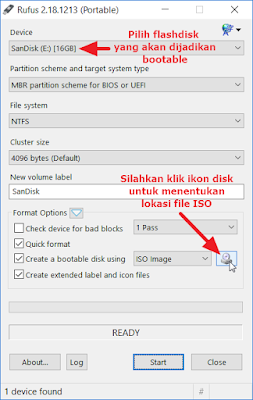
\includegraphics[scale=0.4]{figures/1.png}
	\caption{Proses membuat bootable}
	\label{labelgambar1}
	\end{figure}

  \item Maka akan terbuka jendela file explorer. Kemudian, cari lokasi file file ISO Windows 10 itu berada. jika sudah ketemu lokasi file ISO nya, klik satu kali pada file ISO tersebut dan kemudian tekan tombol Open. ( pada gambar \ref{labelgambar2} )
       \begin{figure}[h!]
	\centering
	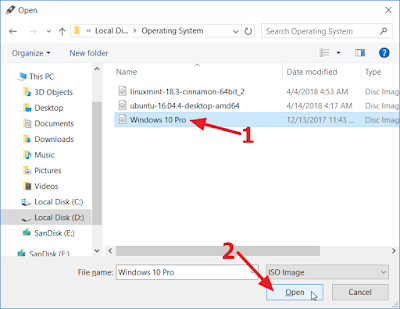
\includegraphics[scale=0.4]{figures/2.png}
	\caption{Proses pemilihan file ISO}
	\label{labelgambar2}
	\end{figure}

  \item Secara otomatis nama device flashdisk akan berubah. Anda bisa mengubah nama flashdisk sesuai dengan yang Anda inginkan pada kolom New volume label. Jika nama flashdisk sudah diganti atau Anda tidak ingin mengganti nama flashdisk, silahkan klik tombol Start untuk memulai proses pembuatan bootable flashdisk Windows 10. ( pada gambar \ref{labelgambar3} )
      \begin{figure}[h!]
	\centering
	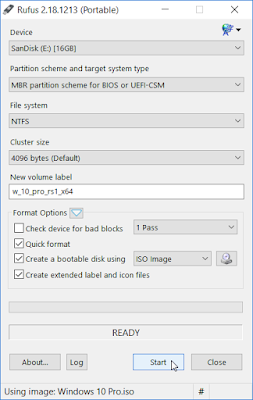
\includegraphics[scale=0.4]{figures/3.png}
	\caption{Proses pembuatan bootable}
	\label{labelgambar3}
	\end{figure}

  \item Akan muncul jendela peringatan, bahwa semua data yang terdapat di flashdisk akan dihapus. Maka dari itu, pastikan Anda untuk memindahkan terlebih dahulu data penting yang terdapat pada flashdisk. Jika sudah memindahkan data penting pada flashdisk, silahkan klik tombol OK. ( pada gambar \ref{labelgambar4} )
      \begin{figure}[h!]
	\centering
	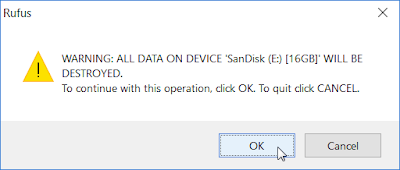
\includegraphics[scale=0.4]{figures/4.png}
	\caption{Proses pembuatan bootable}
	\label{labelgambar4}
	\end{figure}

  \item Maka proses pembuatan bootable flashdisk Windows 10 dimulai, tunggulah beberapa saat sampai prosesnya selesai. Biasanya hanya memakan waktu 10 menit, itu juga tergantung pada ukuran file ISO dan spesifikasi laptop atau komputer Anda. ( pada gambar \ref{labelgambar5} )
       \begin{figure}[h!]
	\centering
	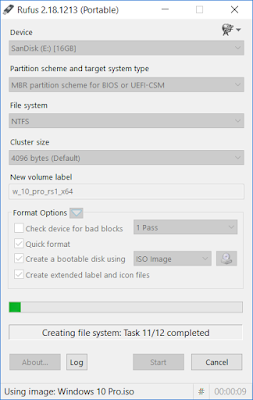
\includegraphics[scale=0.4]{figures/5.png}
	\caption{Proses pembuatan bootable}
	\label{labelgambar5}
	\end{figure}

  \item Jika progres bar berwarna hijau sudah penuh dan terdapat tulisan READY dibawahnya, itu menandakan flashdisk Anda sudah selesai di bootable dan siap digunakan sebagai media instalasi untuk memasang Windows 10 pada laptop atau komputer. Klik tombol Close untuk keluar dari aplikasi Rufus. ( pada gambar \ref{labelgambar6} )
      \begin{figure}[h!]
	\centering
	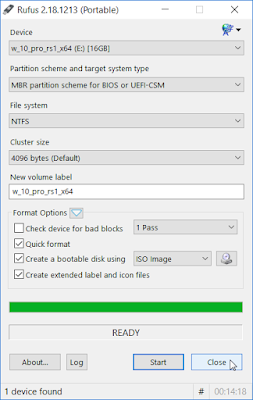
\includegraphics[scale=0.4]{figures/6.png}
	\caption{Proses pembuatan bootable}
	\label{labelgambar6}
	\end{figure}
\end{enumerate}

\subsection{Tahap Eksekusi}
\begin{enumerate}
  \item Pertama-tama matikan PC/laptop anda kemudian colok/masukkan Bootable USB Windows 10 yang sudah anda buat ke port USB PC/Laptop anda.
  \item Setelah itu masuk ke BIOS, caranya dengan menekan Tombol F2 pada keybord segera setelah menyalakan PC/laptop anda. Tombol untuk masuk ke BIOS ini bisa saja bukan F2, tetapi ada beberapa tombol lain tergantung PC/Laptop anda seperti F8, DEL, ESC, dll.
  \item Setelah anda masuk ke BIOS silahkan pergi ke Tab Boot, disana anda akan melihat beberapa daftar perangkat seperti Hardisk (HDD), DVD, Flashdisk, dll. Anda dapat perhatikan bahwa yang berada pada urutan pertama adalah Hardisk (HDD) PC/Laptop anda, sedangkan Flashdisk yang merupakan Bootable USB Windows 10 berada di urutan sekian. Hal yang harus anda lakukan adalah memindahkan Flashdisk yang merupakan Bootable USB anda ke urutan pertama pada Boot Priority. Hal ini bertujuan agar ketika PC/laptop anda dinyalakan maka Bootable USB anda akan langsung dieksekusi sehingga proses install Windows 10 sudah dapat dilakukan. Untuk memindahkan Flashdisk anda ke urutan pertama pada Boot Priority anda dapat menggunakan tombol – dan + sebagai navigasi untuk menggesernya keatas atau kebawah. Pada jenis PC/Laptop tertentu juga biasa digunakan F5 dan F6 sebagai tombol navigasi.
  \item Jika anda sudah memindahkan Flashdisk anda pada urutan pertama, silahkan simpan pengaturan BIOS anda dengan menekan F10 pada keyboard.
  \item Cara lain untuk mengakses Bootable USB adalah dengan menekan F12 segera saat PC/Laptop anda dinyalakan, kemudian pilih dan tekan enter pada Flashdisk anda. Tetapi tidak semua jenis PC/Laptop memiliki fungsi tombol ini.
\end{enumerate}

\subsection{Proses Instalasi}
\begin{enumerate}
  \item Setelah melakukan setting BIOS, kemudian simpan pengaturan BIOS anda dengan menekan tombol F10 pada keyboard.
  \item PC/Laptop anda akan restart, kemudian akan muncul sebuah teks dengan tulisan Press any key to boot from CD or USB…. Silahkan tekan tombol apa saja pada keyboard pada saat teks tersebut muncul. ( pada gambar \ref{labelgambar7})
      \begin{figure}[h!]
	\centering
	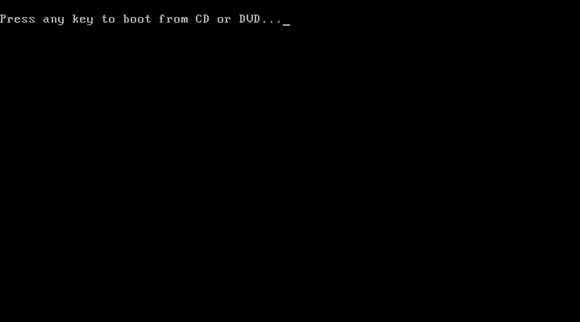
\includegraphics[scale=0.4]{figures/1.jpg}
	\caption{Proses Install Windows 10}
	\label{labelgambar7}
	\end{figure}
  \item Setelah itu akan muncul jendela Setup Windows 10. Pada tampilan awal anda harus memilih bahasa, format Waktu, dan Keyborad Input. Pada piihan bahasa silahkan pilih English, pada Format waktu silahkan pilih Indonesia, dan pada keyboard input silahkan pilih US dikarenakan type keyboard yang beredar di Indonesia adalah type US. Kemudian klik Next. ( pada gambar \ref{labelgambar8})
      \begin{figure}[h!]
	\centering
	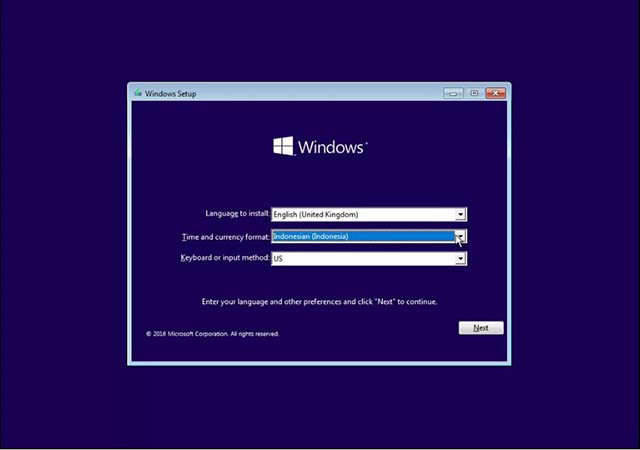
\includegraphics[scale=0.4]{figures/2.JPG}
	\caption{Proses Install Windows 10}
	\label{labelgambar8}
	\end{figure}
  \item Pada jendela selanjutnya yang muncul silahkan klik Install Now.
  \item Jika anda diminta memasukkan Product key silahkan masukkan product key yang anda miliki kemudian klik Next. Tapi jika tidak punya silahkan abaikan dengan klik I don’t have a product key. ( pada gambar \ref{labelgambar9})
      \begin{figure}[h!]
	\centering
	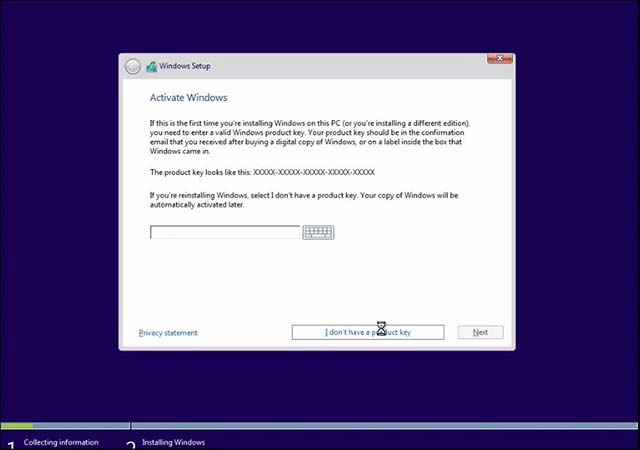
\includegraphics[scale=0.4]{figures/3.JPG}
	\caption{Proses Install Windows 10}
	\label{labelgambar9}
	\end{figure}
\item Pada bagian license terms, centang/ceklis pada checkbox I accept the license terms kemudian klik Next. (pada gambar \ref{labelgambar10})
    \begin{figure}[h!]
	\centering
	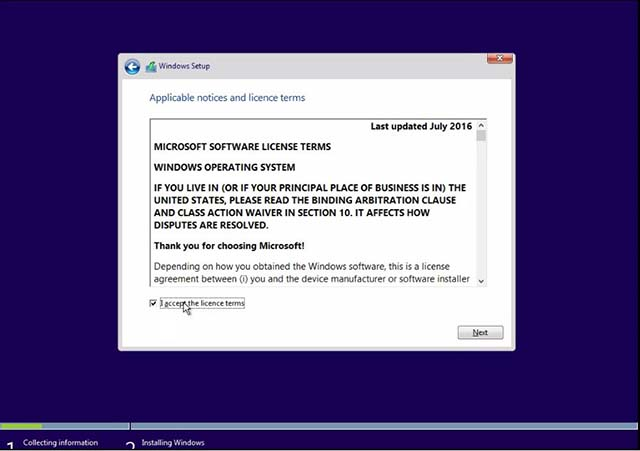
\includegraphics[scale=0.4]{figures/4.JPG}
	\caption{Proses Install Windows 10}
	\label{labelgambar10}
	\end{figure}
\item Pada jendela selanjutnya anda harus memilih metode install. Terdapat dua pilihan yaitu Upgrade dan Custom (Advance). Pada kasus ini silahkan pilih Custom karena akan melakukan clean install dan menghapus Windows yang sebelumnya. Anda dapat memilih Upgrade jika hendak memperbaharui Windows 10 yang sudah ada sebelumnya tanpa menghapus data-data dan pengaturan Windowsnya. (pada gambar \ref{labelgambar11})
    \begin{figure}[h!]
	\centering
	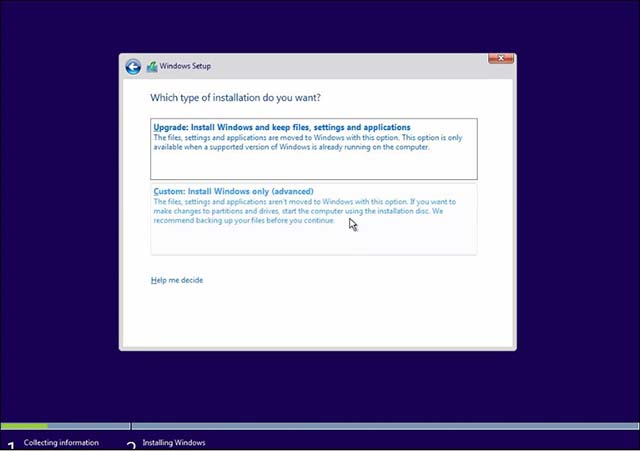
\includegraphics[scale=0.4]{figures/5.JPG}
	\caption{Proses Install Windows 10}
	\label{labelgambar11}
	\end{figure}
\item Selanjutnya anda akan masuk ke pengaturan partisi Hardisk. Disini anda harus berhati-hati dalam menghapus partisi untuk menghindari hilangnya data anda.
\item Jika PC/Laptop anda diinstall untuk pertama kalinya maka tentu saja belum terdapat pembagian partisi pada Hardisknya (Unalocated Space). Anda dapat membuat partisi baru dengan klik New. Anda harus membuat beberapa partisi sesuai keinginan anda, tetapi yang harus anda perhatikan adalah anda harus membuat sebuah partisi tempat dimana Windows 10 akan diinstall. Jika anda akan melakukan install Ulang atau pada PC/laptop anda sudah terdapat Windows sebelumnya, maka anda harus mneghapus partisi Windows yang sebelumnya. Silahkan klik pada Partisi Windows sebelumnya kemudian klik Delete. Jika anda salah hapus partisi maka anda akan kehilangan data anda. Setelah anda menghapus partisi Windows sebelumnya silahkan buat partisi baru dengan klik New. Setelah anda membuat partisi baru silahkan klik pada partisi baru yang sudah anda buat kemudian klik Next.
\item Proses Install Windows 10 akan berlangsung, silakan tunggu sampai prosesnya selesai. Proses ini akan membutukan waktu 20-30 menit tergantung kecepatan PC/laptop anda. Pada proses ini PC/Laptop anda akan restart beberapa kali. Perlu diperhatikan, saat PC/laptop anda restart dan muncul teks Press any key to boot from CD or USB… seperti pada gambar \ref{labelgambar7} maka kali ini biarakan saja dan jangan tekan tombol apapun karena jika anda menekan tombol apa saja maka proses install akan terulang dari awal. ( pada gambar \ref{labelgambar12})
    \begin{figure}[h!]
	\centering
	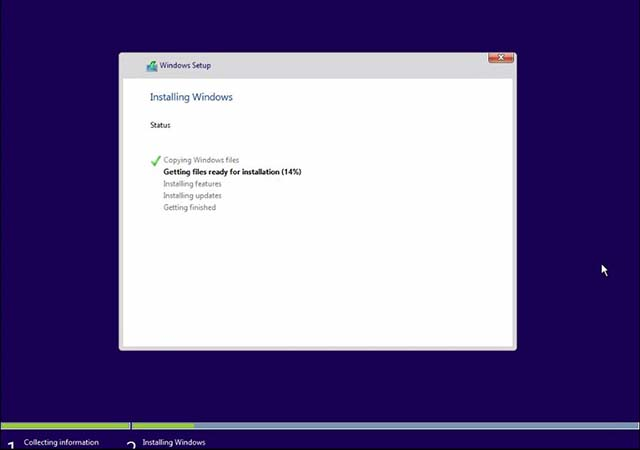
\includegraphics[scale=0.4]{figures/6.JPG}
	\caption{Proses Install Windows 10}
	\label{labelgambar12}
	\end{figure}
\item Setelah selesai, maka diperlukan beberapa waktu untuk persipan sebelum memasuki proses konfigurasi Windows 10 anda.
\item Pada proses konfigurasi Windows 10, maka yang pertama yang harus anda lakukan adalah memasukkan username dan password. Password ini akan digunakan untuk login pada Windows 10 anda nantinya. Anda dapat mengatur password dan boleh juga dikosongkan. Disini terdapat tiga isian ketika anda hendak mengatur password yaitu anda harus memasukkan password, kemudian mengulanginya pada isian kedua, kemudian mengisi password hint yang merupakan petunjuk yang akan muncul jika anda lupa password. Kemudian klik Next. (pada gambar \ref{labelgambar13})
    \begin{figure}[h!]
	\centering
	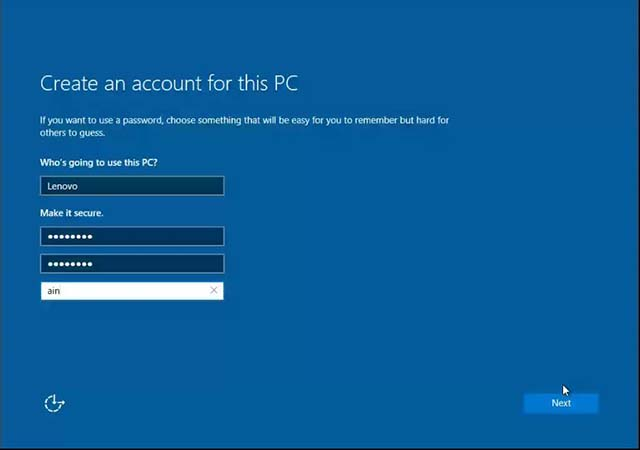
\includegraphics[scale=0.4]{figures/7.JPG}
	\caption{Proses Install Windows 10}
	\label{labelgambar13}
	\end{figure}
\item Selanjutnya pada jendela Meet Cortana, silahkan pilih apakah ingin menggunakan Cortana atau tidak. Klik Use Cortana jika ingin mengaktifkan Cortana dan klik Not Now jiak ingin mengabaikannnya. Tapi berhubung karena di Indonesia belum sepenuhnyya mendapat dukungan Cortana maka sebaiknya abaikan saja. (pada gambar \ref{labelgambar14})
    \begin{figure}[h!]
	\centering
	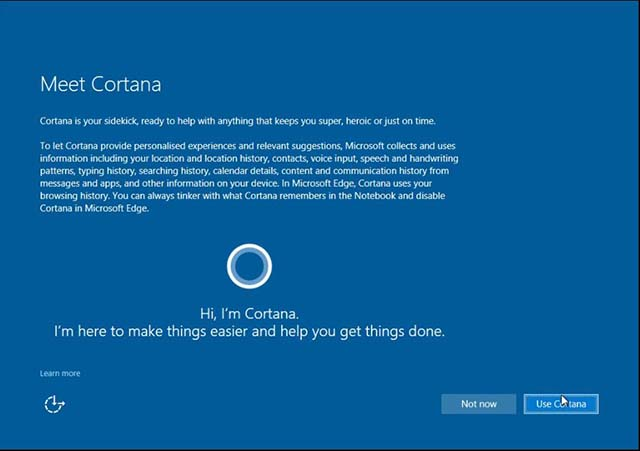
\includegraphics[scale=0.4]{figures/8.JPG}
	\caption{Proses Install Windows 10}
	\label{labelgambar14}
	\end{figure}
\item Selanjutnya tunggu sampai Finalisasi settings selesai.
(pada gambar \ref{labelgambar15})
    \begin{figure}[h!]
	\centering
	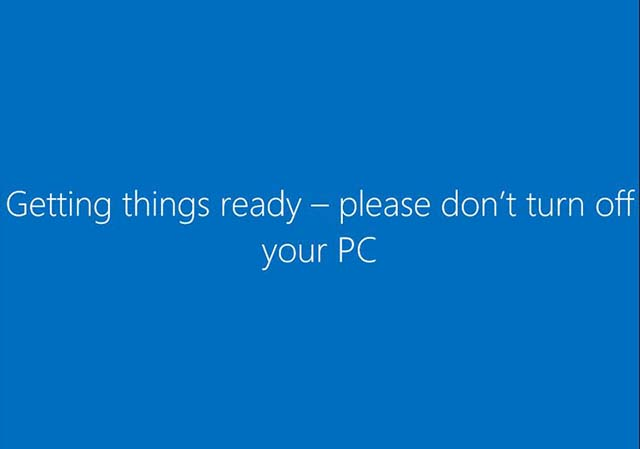
\includegraphics[scale=0.4]{figures/9.JPG}
	\caption{Proses Install Windows 10}
	\label{labelgambar15}
	\end{figure}
\item Silahkan login pada Windows 10 anda menggunakan password yang sudah anda atur sebelumnya.
\item Setelah selesai maka proses install dan konfigurasi Windows 10 sudah selesai dan anda sudah dapat menggunakan Windows 10 pada PC/laptop anda. (pada gambar \ref{labelgambar16})
    \begin{figure}[h!]
	\centering
	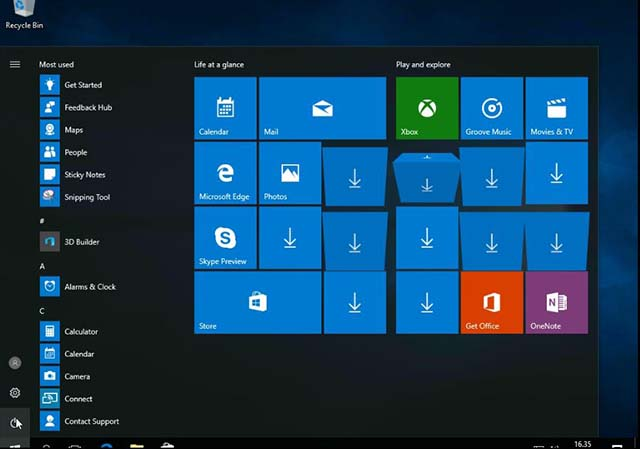
\includegraphics[scale=0.4]{figures/10.JPG}
	\caption{Proses Install Windows 10}
	\label{labelgambar16}
	\end{figure}
\end{enumerate}

Setelah anda menginstall Windows 10, maka hal yang harus anda lakukan adalah menginstall Driver PC/laptop anda agar kinerjanya maksimal. Setelah itu silahkan install aplikasi yang anda butuhkan.
 